\documentclass{beamer}

\usetheme{simple}

\usepackage{scalerel,xparse}
\usepackage{lmodern}
\usepackage[scale=2]{ccicons}
\usepackage{ulem}
\usepackage{tikz}
\usetikzlibrary{positioning,calc,automata}
\usepackage{algorithm}
\usepackage{algorithmic}
\usepackage{caption}
\usepackage{listings}
\usepackage{xcolor}

% Watermark background (simple theme)
\setlength{\parindent}{0cm}
\setwatermark{
\includegraphics[height=8cm]{img/amogus.png}}


\title{\sout{CSC363} CSC369 Tutorial 6}
\subtitle{hope tomorrow's paul is feeling better!\\ (paul, having a headache and sick, on feb 23, while preparing slides)}
\date{\today}
\author{Paul ``sushi{\textunderscore}enjoyer'' Zhang}
\institute{University of Amogus}

\NewDocumentCommand\emojisushi{}{
    
\includegraphics{img/1f363.png}
}
\NewDocumentCommand\emojiflushed{}{
    
\includegraphics[scale=0.05]{img/1f633.png}
}  
\NewDocumentCommand\emojimoyai{}{
    
\includegraphics{img/1f5ff.png}
}   

\begin{document}

\maketitle

\begin{frame}{Learning objectives this tutorial}
By the end of this tutorial, you should...
\begin{itemize}
\item Once again have CSIS (or whatever law enforcement for copyright violations in your jurisdiction) come to your house due to [REDACTED].
\item Have recalled the formal definition of a Turing machine, and have built one in Minecraft (or any other Turing-complete game)
\item Understand the formal definition of a multi-tape Turing machine, and have built one again in Minecraft (or any other Turing-complete game).
\item Understand the formal definition of a nondeterministic Turing machine.
\item Be infuriated by any further mentioning of computability, because we are completely done with that chapter of our lives.\footnote{If you hate computability, don't open assignment 3! (too bad you're forced to ;-;)}
\end{itemize}
\end{frame}

\begin{frame}{More unaffordable textbooks! yay :/}
\begin{figure}[h]
\centering
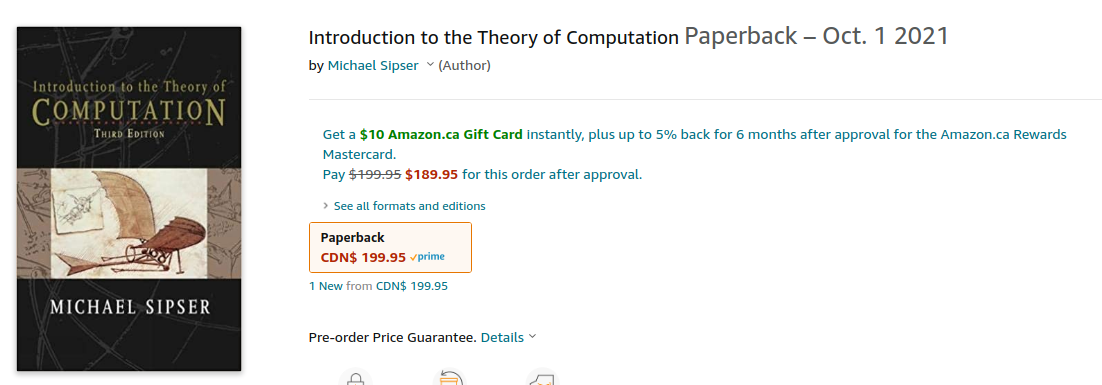
\includegraphics[width=9cm]{img/amazon.png}

i'm broke from spending money on sushi. i can't afford this textbook.
\end{figure}
Again, it's worth a read! you'll go over cool stuff like
\begin{itemize}
\item What really is a Turing machine? (3.1)
\item What are multi-tape and nondeterministic Turing machines? Why are they equivalent to Turing machines? (3.2)
\item What does $f(n) = O(g(n))$ mean again? What does $P$ mean? (7.1, 7.2)
\item Why didn't we use this textbook earlier? (69.420)
\end{itemize}
\end{frame}


\begin{frame}{Turing machines are back! :D}
Hope you remember what a Turing machine is! 

\begin{center}
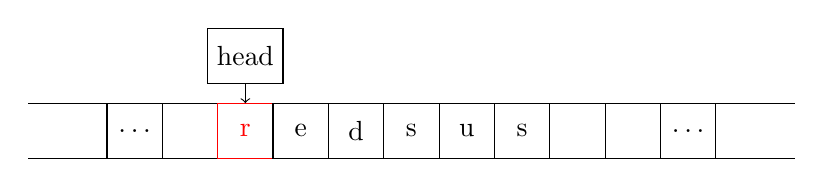
\begin{tikzpicture}[every node/.style={block},
        block/.style={minimum height=2em,minimum width=2em,outer sep=0pt,draw,rectangle,node distance=0pt}]
   \node (R1) {$\ldots$};
   \node (R2) [right=of R1] {$\square$};
   \node (R3) [right=of R2, color=red] {r};
   \node (R4) [right=of R3] {e};
   \node (R5) [right=of R4] {d};
   \node (R6) [right=of R5] {s};
   \node (R7) [right=of R6] {u};
   \node (R8) [right=of R7] {s};
   \node (R9) [right=of R8] {\emojiflushed};
   \node (R10) [right=of R9] {$\square$};
   \node (R11) [right=of R10] {$\ldots$};
   \node (HEAD) [above = 0.25cm of R3] {head};
   \draw[->] (HEAD) -- (R3);
   \draw (R1.north west) -- ++(-1cm,0) (R1.south west) -- ++ (-1cm,0);
   \draw (R11.north east) -- ++(1cm,0) (R11.south east) -- ++ (1cm,0);
\end{tikzpicture}
\end{center}
This Turing machine is sus \emojiflushed it only has one tape. what if we had multiple tapes?
\begin{center}
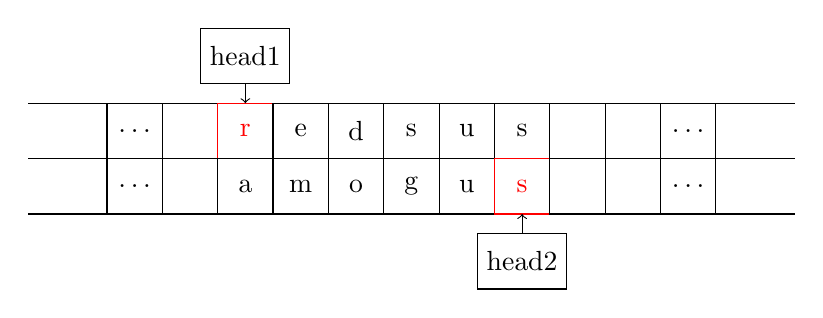
\begin{tikzpicture}[every node/.style={block},
        block/.style={minimum height=2em,minimum width=2em,outer sep=0pt,draw,rectangle,node distance=0pt}]
   \node (R1) {$\ldots$};
   \node (R2) [right=of R1] {$\square$};
   \node (R3) [right=of R2, color=red] {r};
   \node (R4) [right=of R3] {e};
   \node (R5) [right=of R4] {d};
   \node (R6) [right=of R5] {s};
   \node (R7) [right=of R6] {u};
   \node (R8) [right=of R7] {s};
   \node (R9) [right=of R8] {\emojiflushed};
   \node (R10) [right=of R9] {$\square$};
   \node (R11) [right=of R10] {$\ldots$};
   \draw (R1.north west) -- ++(-1cm,0) (R1.south west) -- ++ (-1cm,0);
   \draw (R11.north east) -- ++(1cm,0) (R11.south east) -- ++ (1cm,0);
   \node (R12) [below=of R1] {$\ldots$};
   \node (R13) [right=of R12] {$\square$};
   \node (R14) [right=of R13] {a};
   \node (R15) [right=of R14] {m};
   \node (R16) [right=of R15] {o};
   \node (R17) [right=of R16] {g};
   \node (R18) [right=of R17] {u};
   \node (R19) [right=of R18, color=red] {s};
   \node (R20) [right=of R19] {\emojiflushed};
   \node (R21) [right=of R20] {$\square$};
   \node (R22) [right=of R21] {$\ldots$};
   \draw (R12.north west) -- ++(-1cm,0) (R12.south west) -- ++ (-1cm,0);
   \draw (R22.north east) -- ++(1cm,0) (R22.south east) -- ++ (1cm,0);
   \node (HEAD1) [above = 0.25cm of R3] {head1};
   \draw[->] (HEAD1) -- (R3);
   \node (HEAD2) [below = 0.25cm of R19] {head2};
   \draw[->] (HEAD2) -- (R19);
\end{tikzpicture}
\end{center}

\end{frame}

\begin{frame}{Turing machines are back! :D}
\begin{center}
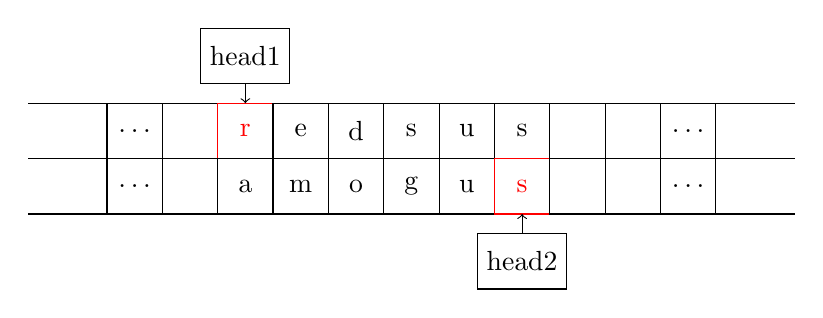
\begin{tikzpicture}[every node/.style={block},
        block/.style={minimum height=2em,minimum width=2em,outer sep=0pt,draw,rectangle,node distance=0pt}]
   \node (R1) {$\ldots$};
   \node (R2) [right=of R1] {$\square$};
   \node (R3) [right=of R2, color=red] {r};
   \node (R4) [right=of R3] {e};
   \node (R5) [right=of R4] {d};
   \node (R6) [right=of R5] {s};
   \node (R7) [right=of R6] {u};
   \node (R8) [right=of R7] {s};
   \node (R9) [right=of R8] {\emojiflushed};
   \node (R10) [right=of R9] {$\square$};
   \node (R11) [right=of R10] {$\ldots$};
   \draw (R1.north west) -- ++(-1cm,0) (R1.south west) -- ++ (-1cm,0);
   \draw (R11.north east) -- ++(1cm,0) (R11.south east) -- ++ (1cm,0);
   \node (R12) [below=of R1] {$\ldots$};
   \node (R13) [right=of R12] {$\square$};
   \node (R14) [right=of R13] {a};
   \node (R15) [right=of R14] {m};
   \node (R16) [right=of R15] {o};
   \node (R17) [right=of R16] {g};
   \node (R18) [right=of R17] {u};
   \node (R19) [right=of R18, color=red] {s};
   \node (R20) [right=of R19] {\emojiflushed};
   \node (R21) [right=of R20] {$\square$};
   \node (R22) [right=of R21] {$\ldots$};
   \draw (R12.north west) -- ++(-1cm,0) (R12.south west) -- ++ (-1cm,0);
   \draw (R22.north east) -- ++(1cm,0) (R22.south east) -- ++ (1cm,0);
   \node (HEAD1) [above = 0.25cm of R3] {head1};
   \draw[->] (HEAD1) -- (R3);
   \node (HEAD2) [below = 0.25cm of R19] {head2};
   \draw[->] (HEAD2) -- (R19);
\end{tikzpicture}
\end{center}
This 2-tape Turing machine will read in 2 symbols at once (as a 2-tuple), consult the current state, then output the following:
\begin{enumerate}
\item Next state to transition towards;
\item Symbol to write back via head1, and direction to move head1;
\item Symbol to write back via head2, and direction to move head2.
\end{enumerate}
\end{frame}



\begin{frame}{Greek letters are back! D:}
Do you like formal definitions? If you don't, too bad :(

\textbf{Task:} Recall that a Turing machine (the mathematical object) is an $8$-tuple $(Q, \Sigma, \Gamma, \delta, q_0, q_\text{accept}, q_\text{reject}, \square)$ where
\begin{itemize}
\item $Q$ is the (finite) set of states;
\item $\Sigma$ is the input alphabet not containing $\square$;
\item $\Gamma$ is the tape alphabet, and $\square \in \Gamma$ and $\Sigma \subseteq \Gamma$;
\item $\delta: Q \times \Gamma \to Q \times \Gamma \times \{L, R\}$ is the transition function;
\item $q_0 \in Q$ is the starting state;
\item $q_\text{accept}$ is the accept state;
\item $q_\text{reject}$ is the reject state (and $q_\text{reject} \neq q_\text{accept}$);
\item $\square$ is the blank symbol.
\end{itemize}
Familiarize yourself with this definition. Ask any questions you have!
\end{frame}

\begin{frame}{Greek letters are back! D:}
Do you like formal definitions? If you don't, too bad :(

\textbf{Task:} The definition of a $k$-tape Turing machine (the mathematical object) is an $8$-tuple $(Q, \Sigma, \Gamma, \delta, q_0, q_\text{accept}, q_\text{reject}, \square)$ where
\begin{itemize}
\item $Q$ is the (finite) set of states;
\item $\Sigma$ is the input alphabet not containing $\square$;
\item $\Gamma$ is the tape alphabet, and $\square \in \Gamma$ and $\Sigma \subseteq \Gamma$;
\item $\delta: Q \times \Gamma^k \to Q \times \Gamma^k \times \{L, R, -\}^k$ is the transition function;\footnote{$-$ is used to not move the head at all. This additional feature is not in the textbook definition of a $k$-tape Turing machine, but I added it as a user story in my spare time. Don't worry, the computational power is still equivalent.}
\item $q_0 \in Q$ is the starting state;
\item $q_\text{accept}$ is the accept state;
\item $q_\text{reject}$ is the reject state (and $q_\text{reject} \neq q_\text{accept}$);
\item $\square$ is the blank symbol.
\end{itemize}
Compare this with the previous definition. Ask any questions you have!
\end{frame}

\begin{frame}{Greek letters are back! D:}
But how does the $k$-tape Turing machine execute?

Here are the differences between a $k$-tape Turing machine and a regular Turing machine:
\begin{enumerate}
\item In a regular Turing machine, the string input is written on the (only) tape at the start of execution. In a $k$-tape Turing machine, the string input is always written on the first tape.
\item In a $k$-tape Turing machine, we read in $k$ symbols at once, and we output $k$ symbols and $k$ directions from $\{L, R, -\}$, to specify the symbol to write and direction to move for each of the $k$ tapes (where $-$ doesn't move it at all).
\item \texttt{helo\textunderscore fish.jpg} likes multi-tape Turing machines, unlike regular Turing machines.
\begin{figure}[h]
\centering

\includegraphics[width=5cm]{img/helo_fish.jpg}
\end{figure}
\end{enumerate}
\end{frame}

\begin{frame}{Let's try an example!}
I want to construct a 2-tape Turing machine will check if a given binary string is a palindrome. For example, $\emojisushi\emojimoyai\emojisushi\emojisushi\emojisushi\emojisushi\emojimoyai\emojisushi$ is accepted, while $\emojisushi\emojimoyai\emojimoyai\emojimoyai\emojisushi\emojimoyai\emojisushi\emojimoyai$ is not. 

\vspace{2mm}

Say we are given input $\emojisushi\emojisushi\emojimoyai\emojimoyai\emojimoyai\emojisushi\emojisushi$. The Turing machine would start out like so:

\begin{center}
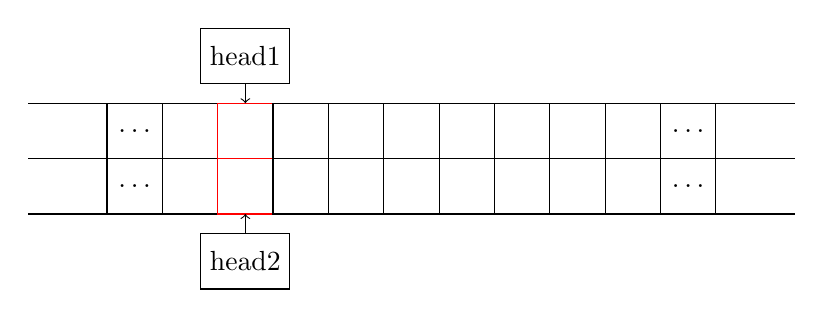
\begin{tikzpicture}[every node/.style={block},
        block/.style={minimum height=2em,minimum width=2em,outer sep=0pt,draw,rectangle,node distance=0pt}]
   \node (R1) {$\ldots$};
   \node (R2) [right=of R1] {$\square$};
   \node (R3) [right=of R2, color=red] {\emojisushi};
   \node (R4) [right=of R3] {\emojisushi};
   \node (R5) [right=of R4] {\emojimoyai};
   \node (R6) [right=of R5] {\emojimoyai};
   \node (R7) [right=of R6] {\emojimoyai};
   \node (R8) [right=of R7] {\emojisushi};
   \node (R9) [right=of R8] {\emojisushi};
   \node (R10) [right=of R9] {$\square$};
   \node (R11) [right=of R10] {$\ldots$};
   \draw (R1.north west) -- ++(-1cm,0) (R1.south west) -- ++ (-1cm,0);
   \draw (R11.north east) -- ++(1cm,0) (R11.south east) -- ++ (1cm,0);
   \node (R12) [below=of R1] {$\ldots$};
   \node (R13) [right=of R12] {$\square$};
   \node (R14) [right=of R13, color=red] {$\square$};
   \node (R15) [right=of R14] {$\square$};
   \node (R16) [right=of R15] {$\square$};
   \node (R17) [right=of R16] {$\square$};
   \node (R18) [right=of R17] {$\square$};
   \node (R19) [right=of R18] {$\square$};
   \node (R20) [right=of R19] {$\square$};
   \node (R21) [right=of R20] {$\square$};
   \node (R22) [right=of R21] {$\ldots$};
   \draw (R12.north west) -- ++(-1cm,0) (R12.south west) -- ++ (-1cm,0);
   \draw (R22.north east) -- ++(1cm,0) (R22.south east) -- ++ (1cm,0);
   \node (HEAD1) [above = 0.25cm of R3] {head1};
   \draw[->] (HEAD1) -- (R3);
   \node (HEAD2) [below = 0.25cm of R14] {head2};
   \draw[->] (HEAD2) -- (R14);
\end{tikzpicture}
\end{center}


\end{frame}

\begin{frame}{Let's try an example!}
\begin{center}
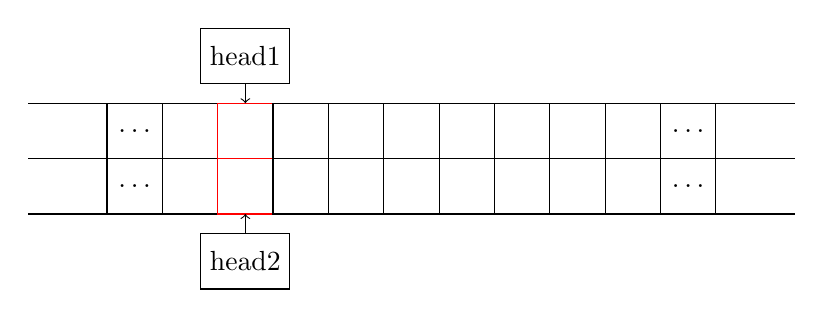
\begin{tikzpicture}[every node/.style={block},
        block/.style={minimum height=2em,minimum width=2em,outer sep=0pt,draw,rectangle,node distance=0pt}]
   \node (R1) {$\ldots$};
   \node (R2) [right=of R1] {$\square$};
   \node (R3) [right=of R2, color=red] {\emojisushi};
   \node (R4) [right=of R3] {\emojisushi};
   \node (R5) [right=of R4] {\emojimoyai};
   \node (R6) [right=of R5] {\emojimoyai};
   \node (R7) [right=of R6] {\emojimoyai};
   \node (R8) [right=of R7] {\emojisushi};
   \node (R9) [right=of R8] {\emojisushi};
   \node (R10) [right=of R9] {$\square$};
   \node (R11) [right=of R10] {$\ldots$};
   \draw (R1.north west) -- ++(-1cm,0) (R1.south west) -- ++ (-1cm,0);
   \draw (R11.north east) -- ++(1cm,0) (R11.south east) -- ++ (1cm,0);
   \node (R12) [below=of R1] {$\ldots$};
   \node (R13) [right=of R12] {$\square$};
   \node (R14) [right=of R13, color=red] {$\square$};
   \node (R15) [right=of R14] {$\square$};
   \node (R16) [right=of R15] {$\square$};
   \node (R17) [right=of R16] {$\square$};
   \node (R18) [right=of R17] {$\square$};
   \node (R19) [right=of R18] {$\square$};
   \node (R20) [right=of R19] {$\square$};
   \node (R21) [right=of R20] {$\square$};
   \node (R22) [right=of R21] {$\ldots$};
   \draw (R12.north west) -- ++(-1cm,0) (R12.south west) -- ++ (-1cm,0);
   \draw (R22.north east) -- ++(1cm,0) (R22.south east) -- ++ (1cm,0);
   \node (HEAD1) [above = 0.25cm of R3] {head1};
   \draw[->] (HEAD1) -- (R3);
   \node (HEAD2) [below = 0.25cm of R14] {head2};
   \draw[->] (HEAD2) -- (R14);
\end{tikzpicture}
\end{center}

We'll program the Turing machine to do the following, at a high level:
\begin{enumerate}
\item Copy the string on the first tape to the second tape.
\item Move head1 to the beginning of the first tape, and head2 to the last character on the second tape.
\item Compare the symbols at head1 and head2. If they are not equal, reject. Else move head1 to the right and head2 to the left. 
\end{enumerate}
\end{frame}

\begin{frame}
\begin{center}
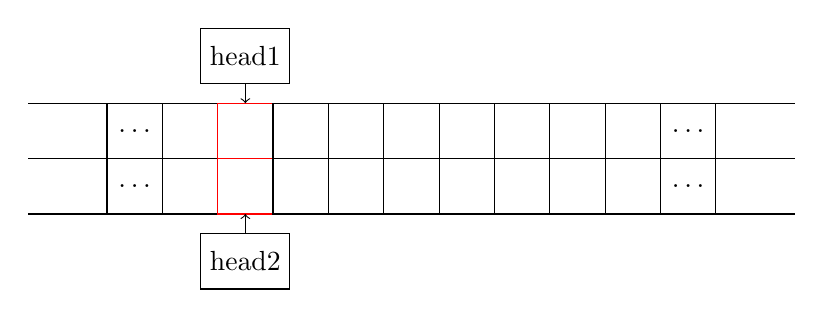
\begin{tikzpicture}[every node/.style={block},
        block/.style={minimum height=2em,minimum width=2em,outer sep=0pt,draw,rectangle,node distance=0pt}]
   \node (R1) {$\ldots$};
   \node (R2) [right=of R1] {$\square$};
   \node (R3) [right=of R2, color=red] {\emojisushi};
   \node (R4) [right=of R3] {\emojisushi};
   \node (R5) [right=of R4] {\emojimoyai};
   \node (R6) [right=of R5] {\emojimoyai};
   \node (R7) [right=of R6] {\emojimoyai};
   \node (R8) [right=of R7] {\emojisushi};
   \node (R9) [right=of R8] {\emojisushi};
   \node (R10) [right=of R9] {$\square$};
   \node (R11) [right=of R10] {$\ldots$};
   \draw (R1.north west) -- ++(-1cm,0) (R1.south west) -- ++ (-1cm,0);
   \draw (R11.north east) -- ++(1cm,0) (R11.south east) -- ++ (1cm,0);
   \node (R12) [below=of R1] {$\ldots$};
   \node (R13) [right=of R12] {$\square$};
   \node (R14) [right=of R13, color=red] {$\square$};
   \node (R15) [right=of R14] {$\square$};
   \node (R16) [right=of R15] {$\square$};
   \node (R17) [right=of R16] {$\square$};
   \node (R18) [right=of R17] {$\square$};
   \node (R19) [right=of R18] {$\square$};
   \node (R20) [right=of R19] {$\square$};
   \node (R21) [right=of R20] {$\square$};
   \node (R22) [right=of R21] {$\ldots$};
   \draw (R12.north west) -- ++(-1cm,0) (R12.south west) -- ++ (-1cm,0);
   \draw (R22.north east) -- ++(1cm,0) (R22.south east) -- ++ (1cm,0);
   \node (HEAD1) [above = 0.25cm of R3] {head1};
   \draw[->] (HEAD1) -- (R3);
   \node (HEAD2) [below = 0.25cm of R14] {head2};
   \draw[->] (HEAD2) -- (R14);
\end{tikzpicture}
\end{center}
1. Copy the string on the first tape to the second tape.
\begin{center}
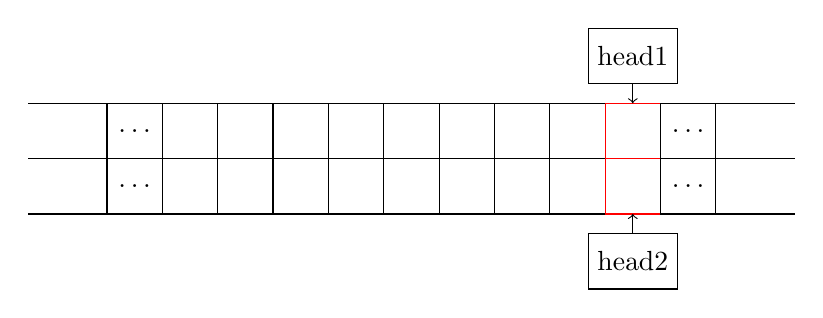
\begin{tikzpicture}[every node/.style={block},
        block/.style={minimum height=2em,minimum width=2em,outer sep=0pt,draw,rectangle,node distance=0pt}]
   \node (R1) {$\ldots$};
   \node (R2) [right=of R1] {$\square$};
   \node (R3) [right=of R2] {\emojisushi};
   \node (R4) [right=of R3] {\emojisushi};
   \node (R5) [right=of R4] {\emojimoyai};
   \node (R6) [right=of R5] {\emojimoyai};
   \node (R7) [right=of R6] {\emojimoyai};
   \node (R8) [right=of R7] {\emojisushi};
   \node (R9) [right=of R8] {\emojisushi};
   \node (R10) [right=of R9, color=red] {$\square$};
   \node (R11) [right=of R10] {$\ldots$};
   \draw (R1.north west) -- ++(-1cm,0) (R1.south west) -- ++ (-1cm,0);
   \draw (R11.north east) -- ++(1cm,0) (R11.south east) -- ++ (1cm,0);
   \node (R12) [below=of R1] {$\ldots$};
   \node (R13) [right=of R12] {$\square$};
   \node (R14) [right=of R13] {$\emojisushi$};
   \node (R15) [right=of R14] {$\emojisushi$};
   \node (R16) [right=of R15] {$\emojimoyai$};
   \node (R17) [right=of R16] {$\emojimoyai$};
   \node (R18) [right=of R17] {$\emojimoyai$};
   \node (R19) [right=of R18] {$\emojisushi$};
   \node (R20) [right=of R19] {$\emojisushi$};
   \node (R21) [right=of R20, color=red] {$\square$};
   \node (R22) [right=of R21] {$\ldots$};
   \draw (R12.north west) -- ++(-1cm,0) (R12.south west) -- ++ (-1cm,0);
   \draw (R22.north east) -- ++(1cm,0) (R22.south east) -- ++ (1cm,0);
   \node (HEAD1) [above = 0.25cm of R10] {head1};
   \draw[->] (HEAD1) -- (R10);
   \node (HEAD2) [below = 0.25cm of R21] {head2};
   \draw[->] (HEAD2) -- (R21);
\end{tikzpicture}
\end{center}
\end{frame}

\begin{frame}
\begin{center}
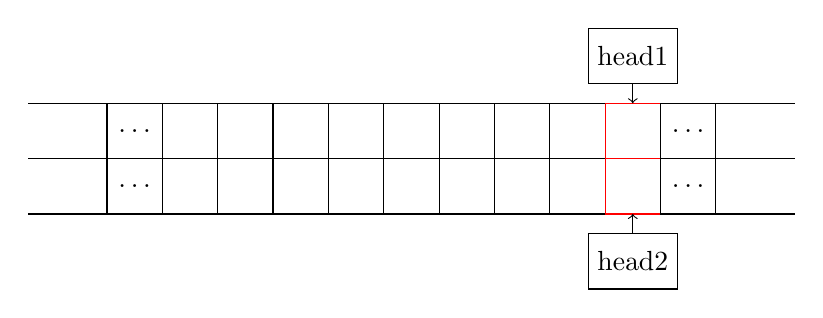
\begin{tikzpicture}[every node/.style={block},
        block/.style={minimum height=2em,minimum width=2em,outer sep=0pt,draw,rectangle,node distance=0pt}]
   \node (R1) {$\ldots$};
   \node (R2) [right=of R1] {$\square$};
   \node (R3) [right=of R2] {\emojisushi};
   \node (R4) [right=of R3] {\emojisushi};
   \node (R5) [right=of R4] {\emojimoyai};
   \node (R6) [right=of R5] {\emojimoyai};
   \node (R7) [right=of R6] {\emojimoyai};
   \node (R8) [right=of R7] {\emojisushi};
   \node (R9) [right=of R8] {\emojisushi};
   \node (R10) [right=of R9, color=red] {$\square$};
   \node (R11) [right=of R10] {$\ldots$};
   \draw (R1.north west) -- ++(-1cm,0) (R1.south west) -- ++ (-1cm,0);
   \draw (R11.north east) -- ++(1cm,0) (R11.south east) -- ++ (1cm,0);
   \node (R12) [below=of R1] {$\ldots$};
   \node (R13) [right=of R12] {$\square$};
   \node (R14) [right=of R13] {$\emojisushi$};
   \node (R15) [right=of R14] {$\emojisushi$};
   \node (R16) [right=of R15] {$\emojimoyai$};
   \node (R17) [right=of R16] {$\emojimoyai$};
   \node (R18) [right=of R17] {$\emojimoyai$};
   \node (R19) [right=of R18] {$\emojisushi$};
   \node (R20) [right=of R19] {$\emojisushi$};
   \node (R21) [right=of R20, color=red] {$\square$};
   \node (R22) [right=of R21] {$\ldots$};
   \draw (R12.north west) -- ++(-1cm,0) (R12.south west) -- ++ (-1cm,0);
   \draw (R22.north east) -- ++(1cm,0) (R22.south east) -- ++ (1cm,0);
   \node (HEAD1) [above = 0.25cm of R10] {head1};
   \draw[->] (HEAD1) -- (R10);
   \node (HEAD2) [below = 0.25cm of R21] {head2};
   \draw[->] (HEAD2) -- (R21);
\end{tikzpicture}
\end{center}
2. Move head1 to the beginning of the first tape, and head2 to the last character on the second tape.
\begin{center}
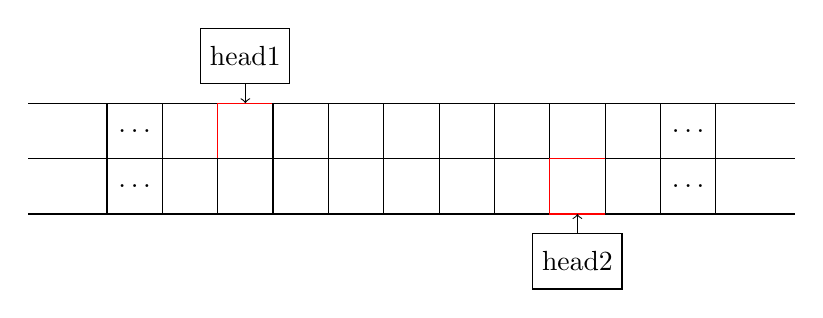
\begin{tikzpicture}[every node/.style={block},
        block/.style={minimum height=2em,minimum width=2em,outer sep=0pt,draw,rectangle,node distance=0pt}]
   \node (R1) {$\ldots$};
   \node (R2) [right=of R1] {$\square$};
   \node (R3) [right=of R2, color=red] {\emojisushi};
   \node (R4) [right=of R3] {\emojisushi};
   \node (R5) [right=of R4] {\emojimoyai};
   \node (R6) [right=of R5] {\emojimoyai};
   \node (R7) [right=of R6] {\emojimoyai};
   \node (R8) [right=of R7] {\emojisushi};
   \node (R9) [right=of R8] {\emojisushi};
   \node (R10) [right=of R9] {$\square$};
   \node (R11) [right=of R10] {$\ldots$};
   \draw (R1.north west) -- ++(-1cm,0) (R1.south west) -- ++ (-1cm,0);
   \draw (R11.north east) -- ++(1cm,0) (R11.south east) -- ++ (1cm,0);
   \node (R12) [below=of R1] {$\ldots$};
   \node (R13) [right=of R12] {$\square$};
   \node (R14) [right=of R13] {$\emojisushi$};
   \node (R15) [right=of R14] {$\emojisushi$};
   \node (R16) [right=of R15] {$\emojimoyai$};
   \node (R17) [right=of R16] {$\emojimoyai$};
   \node (R18) [right=of R17] {$\emojimoyai$};
   \node (R19) [right=of R18] {$\emojisushi$};
   \node (R20) [right=of R19, color=red] {$\emojisushi$};
   \node (R21) [right=of R20] {$\square$};
   \node (R22) [right=of R21] {$\ldots$};
   \draw (R12.north west) -- ++(-1cm,0) (R12.south west) -- ++ (-1cm,0);
   \draw (R22.north east) -- ++(1cm,0) (R22.south east) -- ++ (1cm,0);
   \node (HEAD1) [above = 0.25cm of R3] {head1};
   \draw[->] (HEAD1) -- (R3);
   \node (HEAD2) [below = 0.25cm of R20] {head2};
   \draw[->] (HEAD2) -- (R20);
\end{tikzpicture}
\end{center}
\end{frame}

\begin{frame}
\begin{center}
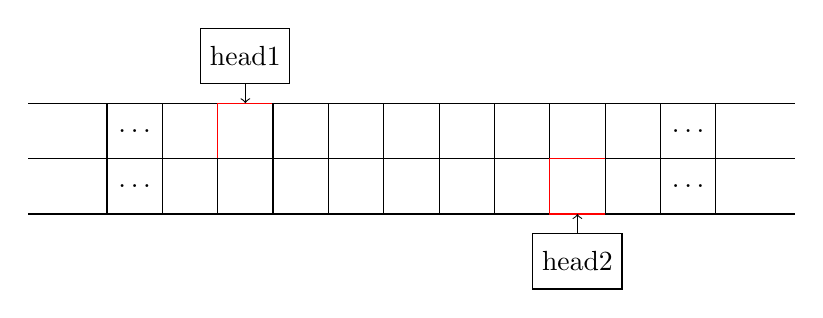
\begin{tikzpicture}[every node/.style={block},
        block/.style={minimum height=2em,minimum width=2em,outer sep=0pt,draw,rectangle,node distance=0pt}]
   \node (R1) {$\ldots$};
   \node (R2) [right=of R1] {$\square$};
   \node (R3) [right=of R2, color=red] {\emojisushi};
   \node (R4) [right=of R3] {\emojisushi};
   \node (R5) [right=of R4] {\emojimoyai};
   \node (R6) [right=of R5] {\emojimoyai};
   \node (R7) [right=of R6] {\emojimoyai};
   \node (R8) [right=of R7] {\emojisushi};
   \node (R9) [right=of R8] {\emojisushi};
   \node (R10) [right=of R9] {$\square$};
   \node (R11) [right=of R10] {$\ldots$};
   \draw (R1.north west) -- ++(-1cm,0) (R1.south west) -- ++ (-1cm,0);
   \draw (R11.north east) -- ++(1cm,0) (R11.south east) -- ++ (1cm,0);
   \node (R12) [below=of R1] {$\ldots$};
   \node (R13) [right=of R12] {$\square$};
   \node (R14) [right=of R13] {$\emojisushi$};
   \node (R15) [right=of R14] {$\emojisushi$};
   \node (R16) [right=of R15] {$\emojimoyai$};
   \node (R17) [right=of R16] {$\emojimoyai$};
   \node (R18) [right=of R17] {$\emojimoyai$};
   \node (R19) [right=of R18] {$\emojisushi$};
   \node (R20) [right=of R19, color=red] {$\emojisushi$};
   \node (R21) [right=of R20] {$\square$};
   \node (R22) [right=of R21] {$\ldots$};
   \draw (R12.north west) -- ++(-1cm,0) (R12.south west) -- ++ (-1cm,0);
   \draw (R22.north east) -- ++(1cm,0) (R22.south east) -- ++ (1cm,0);
   \node (HEAD1) [above = 0.25cm of R3] {head1};
   \draw[->] (HEAD1) -- (R3);
   \node (HEAD2) [below = 0.25cm of R20] {head2};
   \draw[->] (HEAD2) -- (R20);
\end{tikzpicture}
\end{center}
Compare the symbols at head1 and head2. If they are not equal, reject. Else move head1 to the right and head2 to the left. 
\end{frame}

\begin{frame}
I want to construct a 2-tape Turing machine will check if a given binary string is a palindrome. For example, $\emojisushi\emojimoyai\emojisushi\emojisushi\emojisushi\emojisushi\emojimoyai\emojisushi$ is accepted, while $\emojisushi\emojimoyai\emojimoyai\emojimoyai\emojisushi\emojimoyai\emojisushi\emojimoyai$ is not. 

\vspace{2mm}

We'll program the Turing machine to do the following, at a high level:
\begin{enumerate}
\item Copy the string on the first tape to the second tape.
\item Move head1 to the beginning of the first tape, and head2 to the last character on the second tape.
\item Compare the symbols at head1 and head2. If they are not equal, reject. Else move head1 to the right and head2 to the left. 
\end{enumerate}

\textbf{Task:} Formally write this Turing machine down. Remember, a $k$-tape Turing machine (the mathematical object) is an $8$-tuple $(Q, \Sigma, \Gamma, \delta, q_0, q_\text{accept}, q_\text{reject}, \square)$ where
\begin{itemize}
\item $\delta: Q \times \Gamma^k \to Q \times \Gamma^k \times \{L, R, -\}^k$ is the transition function;\footnote{$-$ is used to not move the head at all. This additional feature is not in the textbook definition of a $k$-tape Turing machine, but I added it as a user story in my spare time. Don't worry, the computational power is still equivalent.}
\end{itemize}
\end{frame}

\begin{frame}{They're actually the same!}
Not really. But they're equivalent.
%explaining meme

%in the end
\end{frame}

\begin{frame}{They're actually the same!}
If you're done, convince yourself this problem is much harder using a regular Turing machine.
\end{frame}


\end{document}